\section{Phase 2:  Color Search}

Now the color searching phase will be described.
A small summary is the following: (a) Load the color data structure from disk into the GPU, (b) parse the indexes output of phase 1 from disk and put them in the GPU, (c) search for the color set associated with each index within the GPU, (d) combine all the colors of a sequence together in the GPU, (e) copy the results back from GPU into main memory and write the color sets for each sequence to disk.
Each of these steps, how they are parallelised, and what data structures they produce will be elaborated on in the next section.
Similarly to the index search, the data structures introduced in this section are summarised and explained in a different manner to aid understanding, in Appendix~\ref{app:ColorSearchDataStructures}.

\subsection{Preliminaries and Definitions}

Before discussing the implementations, some mechanisms of how work is done in the GPU need to be introduced.
A unit of work on the GPU is done with a \textit{warp} (or \textit{wave} in AMD terminology).
Each warp in an NVIDIA GPU consists of 32 threads, and 64 in an AMD GPU.
This means that threads within a warp execute at the exact same time under normal conditions.
Threads in a warp can also communicate with one another by sharing the contents of their variables, using what are known as shuffle operations\footnote{\url{https://people.maths.ox.ac.uk/gilesm/cuda/lecs/lec4.pdf}}\footnote{\url{https://docs.nvidia.com/cuda/cuda-c-programming-guide/index.html#warp-shuffle-functions}}\footnote{\url{https://developer.nvidia.com/blog/using-cuda-warp-level-primitives/}}.
For example, if each thread has a variable $X$, this can be broadcasted to all the threads in the same warp.
One common use case of this feature is to get the sum of the variable across the warp.
Another approach is shared memory\footnote{\url{https://docs.nvidia.com/cuda/cuda-c-programming-guide/index.html#shared-memory-variable-declarations}}, which works on the block level.
However, neither shared memory nor blocks will be discussed since they are irrelevant to the rest of the thesis.

A point to remember from Section \ref{sec:Pseudoalignment} is that all $k$-mers in the SBWT are colored, except for dummy $k$-mers.
This means that if a $k$-mer is found in the SBWT, it is colored, and if not, then it is blank.
In this thesis, a colored sequence means refers to sequences that have at least one found $k$-mer, otherwise the sequence will be a \textit{blank sequence}.

\subsection{Loading the Colors}

Now starts the implementation part of this section, with the description of how the colors are loaded.
This data structure is created by Themisto, and needs to be loaded from disk.
The data structure itself is described in Section~\ref{sec:Pseudoalignment}, and all that is added is that the Poppy data structures need to be built for the $\mathit{is\_key\_k\_mer}$ and $\mathit{is\_dense\_marks}$.
This data structure also contains some additional variables such as the number of colors $\mathit{num\_colors}$.
The process is done entirely serially as the items are loaded from the file and the Poppy of the bit-vectors is created serially as well.
These components are then all loaded into GPU memory and kept there until the end.

\subsection{Loading the Indexes}\label{subs:IndexesLoading}

Now the indexes are loaded from disk as they were printed in phase 1.
For this subsection, Figure~\ref{fig:IndexesLoading} shows the final product.
For each sequence the count is taken of how many indexes were found, not found, or are invalid.
Similarly to the first phase, a vector is also created, called the $\mathit{seqs\_before\_newfile}$, which stores a cumulative sum that indicates at which point the algorithm needs to stop considering sequences to be from one file and start considering them as originating from the next file.
A new count is started at the very beginning of a batch or whenever a newline symbol is seen, these symbols being the line feed character '\textbackslash n' for ASCII and a -3 for the binary format.
Again, the boolean format is not suitable for pseudoalignment and cannot be used for phase 2 since this method does not have the indexes.
Similar to reading in phase 1, batching is used with a set maximum number of characters and maximum number of sequences per batch.

For parsing, no special techniques are used.
Characters are read one by one, and for the ASCII format, the na\"ive method of reading one digit and adding it to the previous value multiplied by 10 is used.
This is faster than the C++ standard library, as the standard library implementations usually have some form of error checking involved.
For the binary format, the algorithm simply reads 64 bits at a time.

\begin{figure}[t]
  \centering
  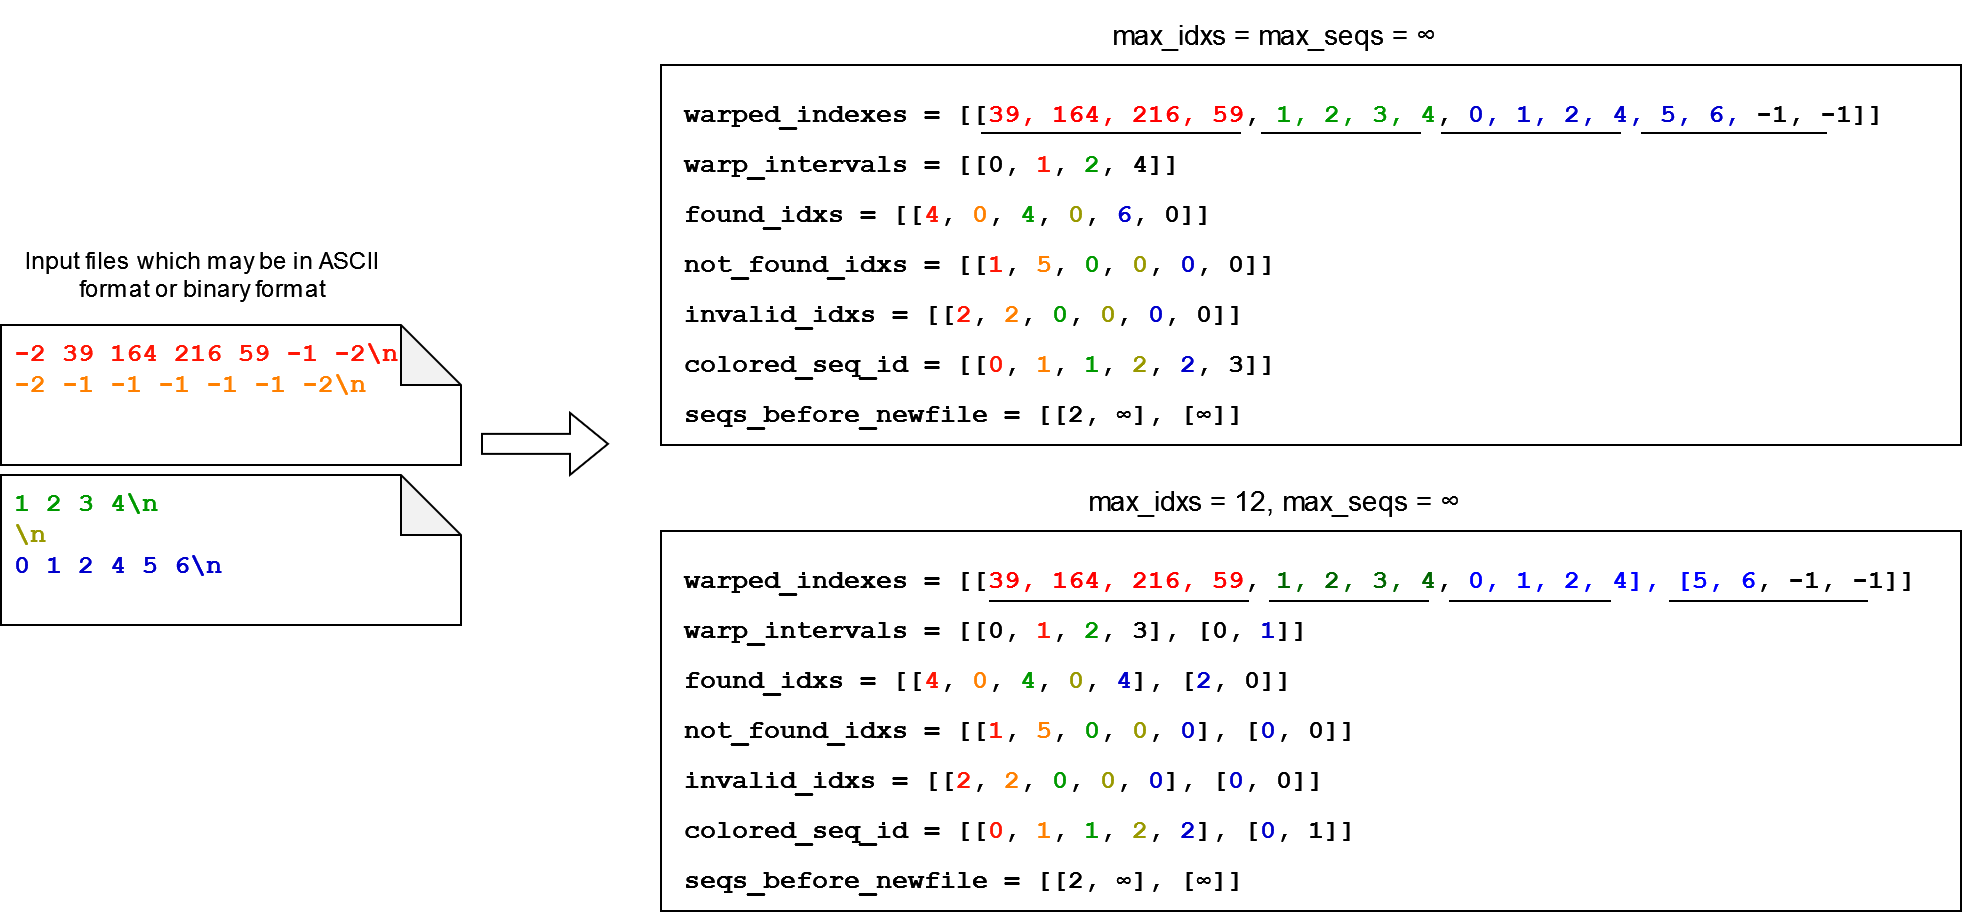
\includegraphics[width=\textwidth]{images/IndexesLoading.png}
  \caption{Example of loading from an ASCII or binary index files and populating the necessary data structures with two different configurations, one where the maximum characters per batch is infinite and one where it is limited to 12, such that the last sequence is broken in two. Note that the last values of the $\mathit{found\_idx}$, $\mathit{not\_found\_idx}$, $\mathit{invalid\_idx}$ and, $\mathit{colored\_seq\_id}$ are because the algorithm needs to consider the next sequence to come.}\label{fig:IndexesLoading}
\end{figure}

Indexes that are not found or invalid are not stored.
This makes the algorithm a lot more efficient, both in terms of time and memory.
The respective counters for the sequence that these indexes belong to are increased, but they are not stored as part of the index list.
Thus, blank sequences effectively take no space, besides the small variables for their counters.
Meanwhile, the indexes of colored sequences are stored contiguously, but between one sequence and the next, padding is used up to the next multiple of the warp size.
This technique and the reasoning for it will be made clearer in Subsection~\ref{subs:ColorSearch}.

Since a sequence may be larger than the warp size, these $\mathit{warped\_indexes}$, as they are called, are then separated via another list called the $\mathit{warp\_intervals}$.
The first entry of this list is always 0, and another entry is added whenever a new sequence causes more $\mathit{warped\_indexes}$ to be added which belong to a new sequence.
Whenever that happens, the new entry which is added will be the cumulative sum of how many warps the algorithm has until the end of that sequence.

Besides the aforementioned variables, another list exists and is called the $\mathit{colored\_seq\_id}$.
This stores an unsigned integer for every sequence, and it indicates which number colored sequence this sequence is.
If a sequence is blank, a $\mathit{colored\_seq\_id}$ is still stored for it, and for convenience, the previous in the list is copied for it, but it might as well be padding as it is later ignored.
This list is then is used in Subsection~\ref{subs:ColorsPrinting}.

\subsection{Searching}\label{subs:ColorSearch}

The next part is the color searching, which is entirely done on the GPU but is split into two kernel calls: Searching and Post Processing.
First, the indexes are copied to the GPU and memory is reserved for the color results.
Note that since blank sequences do not produce any indexes, they also do not use any computations on the GPU later on, thus the algorithm runtime depends on the number of warps spanned by the colored sequences.
Next, the values reserved for the color results are set to 0 using \textit{memset}.
Each thread handles a single index and searches for its color set type, which is sparse or dense, its start index, and its end index, using the same method as Algorithm~\ref{alg:ColorSearch}.
If a thread has a padding index, then it exits immediately.
To do this, a separate GPU functions gets booleans from bitvectors and another extracts a normal u64 from the compact vectors.
The result of this step are the indexes where the color sets start and end within their respective dense or sparse arrays.

The next step of the kernel is to extract and combine the color sets.
First, a small optimisation is performed, which is to get the minimum and maximum color id which exists within the color set of each thread.
To get the minimum present color of a dense color set, the algorithm iterates through the bitvector from the starting point of the color set until the first set bit is found.
Then, to get its maximum, it can simply negate the end index of this color set with the starting index, both of which were found before.
On the other hand, to get these values for sparse colors, one needs to access the sparse color set array and obtain the ones at the start and end indexes to get the minimum and maximum present color id respectively.
Next, an XOR shuffle is performed to broadcast these two values to the other threads inside the warp, so that each thread knows the minimum and maximum color if of all threads within the warp.
To broadcast a value using shuffle, the algorithm needs to perform $log_2(warp\_size)$ steps, as is visualised in Figure~\ref{fig:ShuffleXor}.
Two shuffles need to be performed: one for the minimum and another to broadcast the maximum.
Due to the padding technique when reading the indexes, all threads in each individual warp only contain indexes belonging to a single unique sequence, that is, a warp will not mix colors of different sequences together.

\begin{figure}[t]
  \centering
  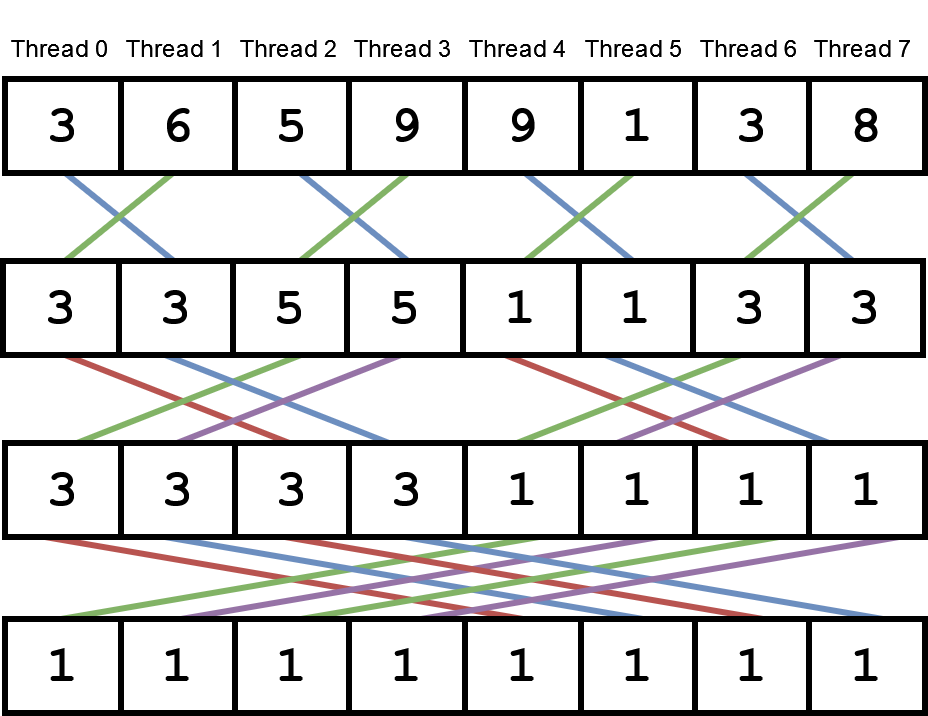
\includegraphics[width=0.7\textwidth]{images/ShuffleXor.png}
  \caption{An example of how data is shared between threads at each step of an XOR shuffle operation to find the min value of the warp. The warp size for this visualisation is 8, hence there are $log_2(8) = 3$ shuffle operations.}\label{fig:ShuffleXor}
\end{figure}

The next step is to iterate through all the colors in the color sets from the minimum and maximum of the warp, and set a boolean value to whether the color exists in the color set of that thread or not.
To get the color presence in the dense array, one can simply do a boolean access in the bitvector at the index of the color.
When it comes to the sparse array, one then needs to go through the array and check if the current color id matches the value in the array.
Luckily the sparse arrays are sorted so the algorithm can do this check in a single step, without going through the whole array for every query, thus going through the whole array only once, as the color presence of every color is checked.

After the color presence of a color is obtained, $\mathit{ballot()}$ is called, where an unsigned integer is created which has as many bits as the warp size, and each thread in the warp sets its respective bit in this integer to 1 if the color is present, and 0 otherwise.
The result of this ballot is broadcasted to all threads in the warp, but it is thread 0 that performs a popcount on this result and stores the color count to device memory.
Notice that this result is at most 32 in the case of NVIDIA devices, and 64 in the case of AMD devices.
This means that a 32-bit integer representation is used for the NVIDIA case, and a 64-bit integer is used for AMD devices.
Furthermore, it also means that the popcount of each of these color counts can be stored in an 8-bit unsigned integer, which is why a list of u8s is used to store these intermediate results, in order to save memory space and thus be able to process more indexes per batch.
The $\mathit{ballot()}$ function is visualised in Figure~\ref{fig:Ballot}, whereas the pseudo code until this point of the color search is found in Algorithm~\ref{alg:GpuColorSearch}.

\begin{figure}[t]
  \centering
  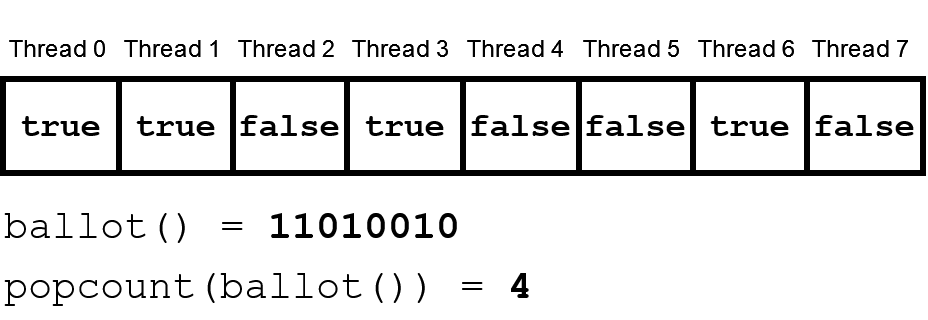
\includegraphics[width=0.7\textwidth]{images/Ballot.png}
  \caption{An example of a ballot operation for a warp of size 8. The ballot operation is called only once in each of the threads, whereas the popcount function on the result of this operation needs to be called by thread 0 only, since this is the one which will be storing the result in this case.}\label{fig:Ballot}
\end{figure}

\begin{algorithm}
	\KwIn{ \\

    $\mathit{warped\_indexes}$

    $\mathit{warp\_size}$

    $\mathit{num\_colors}$

    $\mathit{dense\_arrays}$

    $\mathit{sparse\_arrays}$
	}

  $\mathit{thread\_idx}$ = GPU thread id

  $i$ = $\mathit{warped\_indexes[thread\_idx]}$

  Get $\mathit{start}$, $\mathit{end}$ and $\mathit{is\_dense}$ using $i$ as an input to Algorithm~\ref{alg:ColorSearch}.

  \If{$\mathit{is\_dense}$} {\newline

    $\mathit{min\_id}$ = Traverse $\mathit{dense\_arrays}$ from $\mathit{start}$ to get first set bit

    $\mathit{min\_non\_zero\_color}$ = $\mathit{start}$ - $\mathit{min\_id}$

    $\mathit{max\_non\_zero\_color}$ = $\mathit{end}$ - $\mathit{start}$

  }\Else{ \\

    $\mathit{min\_non\_zero\_color}$ = $\mathit{sparse\_arrays[start]}$

    $\mathit{max\_non\_zero\_color}$ = $\mathit{sparse\_arrays[end - 1]}$
  }

  $\mathit{min\_non\_zero\_color}$ = xor\_shfl($\mathit{min\_non\_zero\_color}$)

  $\mathit{max\_non\_zero\_color}$ = xor\_shfl($\mathit{max\_non\_zero\_color}$)

  $\mathit{array\_idx}$ = $\mathit{start}$

  \ForEach{$\mathit{color\_id}$ \textbf{in} [$\mathit{min\_non\_zero\_color}$ \ldots $\mathit{max\_non\_zero\_color}$]}{

    \If{$\mathit{is\_dense}$} {\newline

      $\mathit{color\_present}$ = ($\mathit{dense\_arrays[array\_idx]}$ = 1)

      ++$\mathit{array\_idx}$

    }\Else{\newline

      $\mathit{color\_present}$ = ($\mathit{sparse\_arrays[array\_idx]}$ = $\mathit{color\_id}$)

      \If{$\mathit{color\_present}$} {\newline

        ++$\mathit{array\_idx}$
      }
    }

    $b$ = ballot($\mathit{color\_present}$)

    \If{$\mathit{thread\_idx}$ \% $\mathit{warp\_size}$ = 0} {\newline
      $\mathit{results}$[$\mathit{num\_colors}$ * $\mathit{thread\_idx}$ / $\mathit{warp\_size}$ + $\mathit{color\_idx}$] = pop\_count($b$)
    }

  }

  \caption{GPU Color Search}\label{alg:GpuColorSearch}
\end{algorithm}

The result of this step is a color count for each color for each warp, where many warps may belong to the same sequence.
Thus, the last step is to postprocess the results by combining the results of the same sequence into a single list.
First, memory is reserved for these u64 results and the warp intervals created in Subsection~\ref{subs:IndexesLoading}, the latter of which can now be copied to the GPU.
Both of these two arrays use the same memory space previously used by the indexes, to maximise memory usage.
Now, one thread is created for every color in every sequence.
Each thread gets a cumulative sum of a single color in the whole sequence and then stores this sum in the new u64s.
These final results can then be copied to CPU memory, as they are now ready for printing.
A visualisation for the post processing step is in Figure~\ref{fig:PostProcessing}.
The disadvantage of this postprocessing method is that if the number of indexes in the colored sequences varies by a lot, then the sequences would produce a disproportionate number of color sets, meaning that some threads would need to do more work.
Luckily, the ballot step of the first phase reduces the work done in this step and the memory required by a factor of 32 on NVIDIA devices and a factor of 64 on AMD devices.
These two factors, that is, both the work done and memory used, is also the reason why it was opted to only put and process colored sequences in the GPU.
Also notice that some threads will only need to only expand the value of the color id from u8 to u64 and store it into the new results, without doing any additions.
Moreover, a flaw of this design is that, given sparse color sets, that is, most colors result in a count of zero, then this design ends up wasting a lot of space, as these zero counts still need to be allocated and also copied back to CPU memory.

\begin{figure}[t]
  \centering
  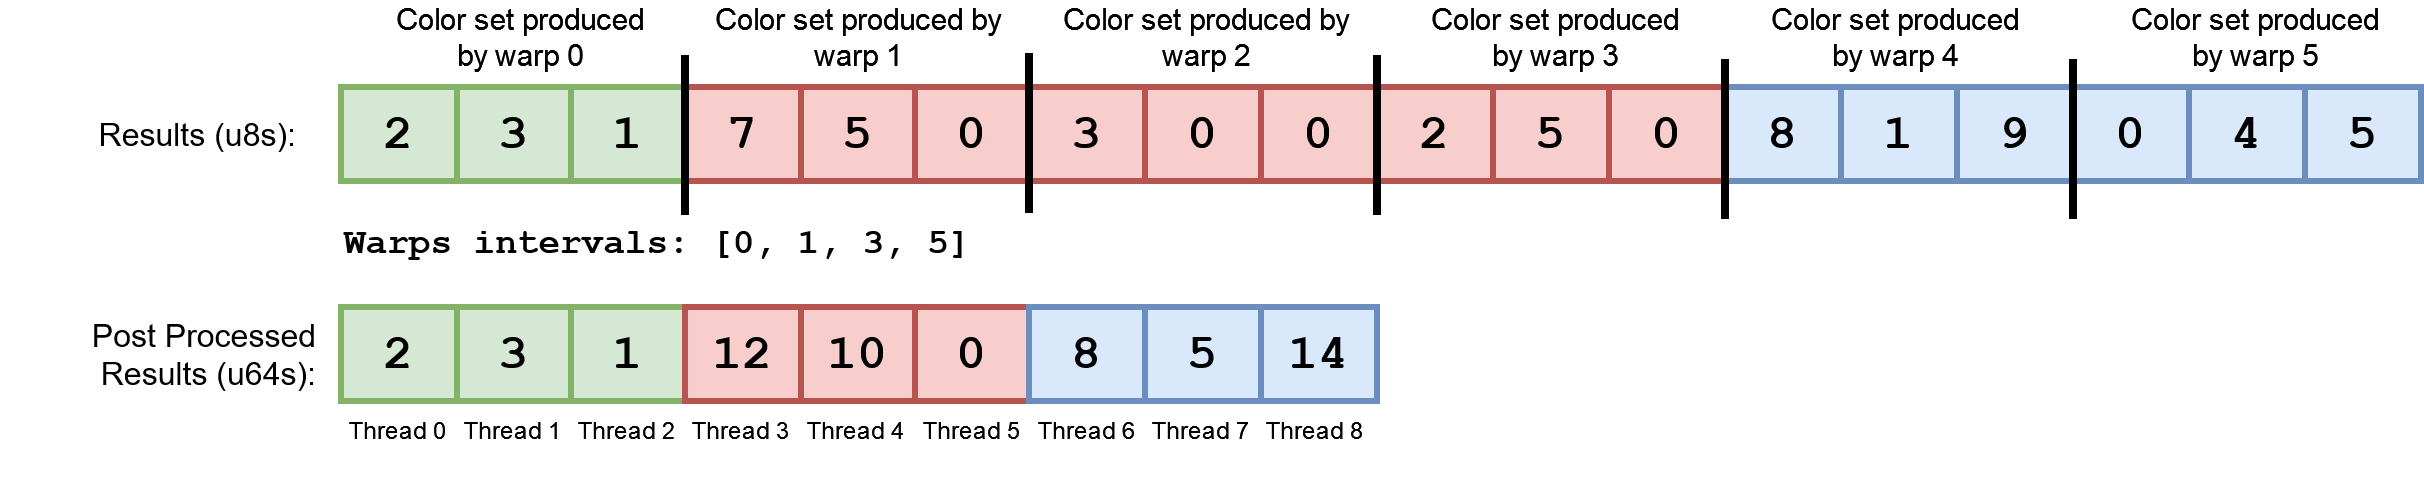
\includegraphics[width=\textwidth]{images/PostProcessing.png}
  \caption{A visualisation of the post processing done on the colors. Each thread handles a single color from each sequence. As a result, some threads may end up doing more work than others if a different number of $k$-mers are found from each sequence. In this case, the middle sequence had more $k$-mers found, which meant that it produced more color sets: 3 warps worth of color sets. Hence, the post processing step does 3 sums for this sequence.}\label{fig:PostProcessing}
\end{figure}

\subsection{Results Printing}\label{subs:ColorsPrinting}

The final step of this last phase is to print the results.
In order to print, besides the colors themselves, the counts for the found, not-found and invalid indexes are provided, alongside the $\mathit{coloured\_seq\_id}$ and the $\mathit{seqs\_before\_newfile}$.
Similarly to the results printing in the first phase, the results are first printed to buffers in parallel and are then printed to disk serially.
For this phase, there are also three output formats: ASCII, binary, and CSV.
In the ASCII format, the colors are printed as space-separated values, where the color id is printed if it appears in the sequence, and each sequence is put on its own line.
Similarly to the previous phase, the boolean format prints each color as a u64 sequentially, where the maximum u64 is used to represent a new line.
These two formats could be seen as the sparse representation outputs, and the CSV is the dense output.
The CSV format prints a comma separated 1 or 0 for each color, where 1 means that the color is present in that sequence and 0 means it is not.
Figure~\ref{fig:ColorsPrinting} shows an example of these three results formats.

When printing to buffers in parallel, each thread handles an equal number of sequences, whether colored or not.
This may lead to some threads doing more work, as colored sequences take much longer to process for the ASCII and binary formats, especially when the color set size is big.
Reads, however, are usually distributed randomly, so the threads should statistically do the same amount of work
Before printing, thresholding is also done in this part.
The contribution of this thesis to this space is the differentiation between thresholding invalid $k$-mers as well as $k$-mers which were not found, the latter of which was included in Themisto.
So the user can choose to ignore one of them, both, or none at all.
Another advantage over Themisto is that the results are always output in ascending order, whereas Themisto may shuffle the results within a single sequence.
Lastly, since a sequence may be split into two batches, the colors and other sequence properties of the last sequence of a batch are copied over to the first sequence of the next batch in order not to lose any information.

\begin{figure}[t]
  \centering
  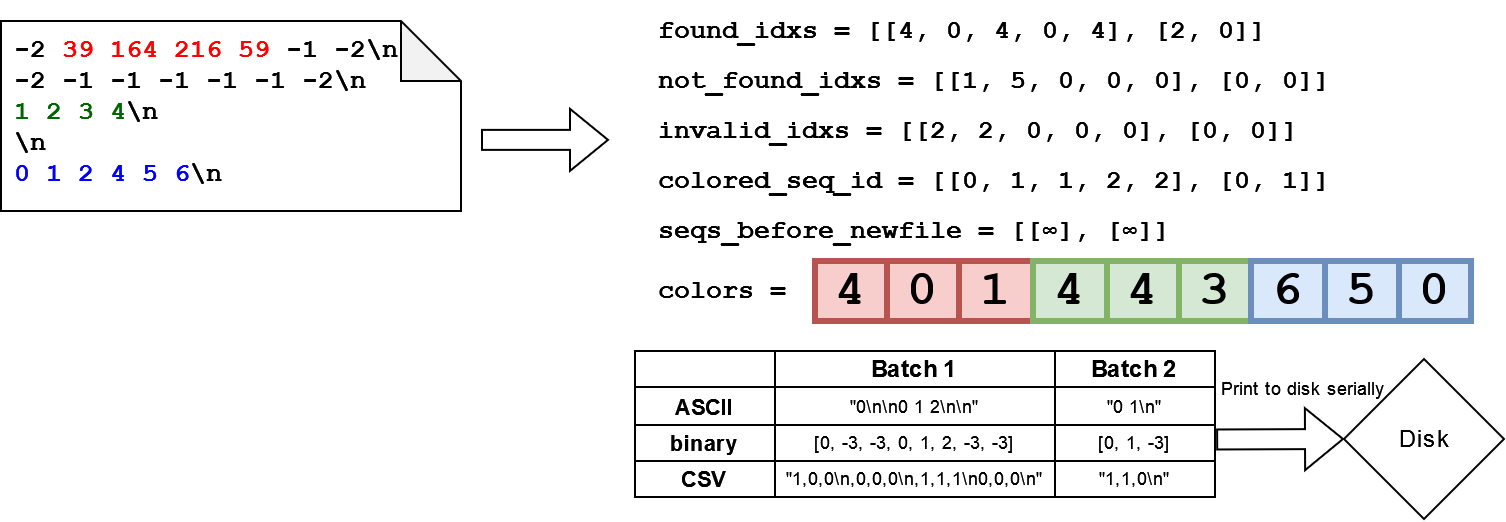
\includegraphics[width=\textwidth]{images/ColorsPrinting.png}
  \caption{A visualisation of the printing of the colors in all three formats. Here, $\tau=0.7$ is used, ignoring the kmers which are not found or invalid.}\label{fig:ColorsPrinting}
\end{figure}
